\textbf{\underline{OZ 10 - De vergelijkingen van Maxwell - Oefening 5:}}
\vspace{0.5cm}

\begin{minipage}{.73\textwidth}
    Een lange cilindrische geleider met straal $R$ draagt een stroom $I$. De stroomdichtheid $J$ is niet uniform over de doorsnede van de geleider, maar variëert volgens $J = br$, met $b$ een positieve constante. Vind een uitdrukking voor het magnetisch veld $B$ $\ldots$
    \begin{enumerate}[(a)]
        \item op een afstand $r_1 < R$,
        \item op een afstand $r_2 > R$.
    \end{enumerate}
\end{minipage}
\begin{minipage}{.23\textwidth}
    \begin{center}
        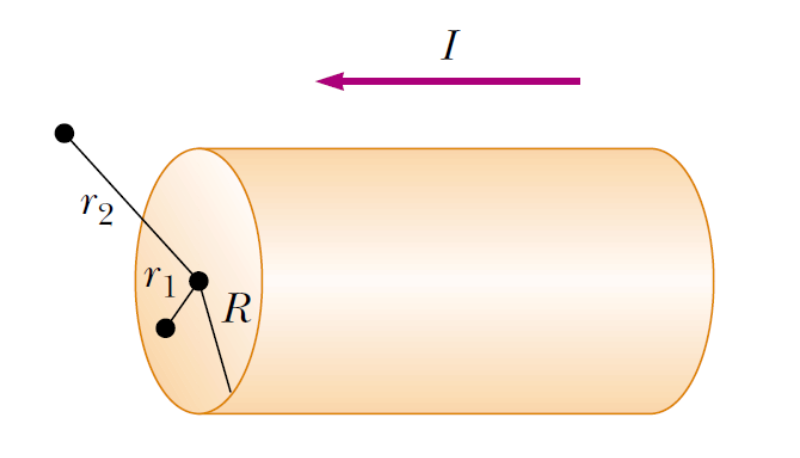
\includegraphics[scale = 0.4]{oz10/resources/Oz10Oef5.png}
    \end{center}
\end{minipage}

\begin{enumerate}[(a)]
    \item 
        \begin{description}[labelwidth=1.5cm, leftmargin=!]
            \item[Geg. :]   
            \item[Gevr. :] 
            \item[Opl. :]   
        \end{description}
    \item
        \begin{description}[labelwidth=1.5cm, leftmargin=!]
            \item[Geg. :]   
            \item[Gevr. :] 
            \item[Opl. :]   
        \end{description}
\end{enumerate}

\vspace{1cm}